\documentclass[conference]{IEEEtran}
\usepackage{times}

% numbers option provides compact numerical references in the text. 
\usepackage[numbers]{natbib}
\usepackage{multicol}
\usepackage[bookmarks=true]{hyperref}
\usepackage{multirow}
\usepackage{graphicx}

\newcommand{\figref}[1]{Fig.~\ref{#1}}



%\pdfinfo{
%   /Author (Homer Simpson)
%   /Title  (Robots: Our new overlords)
%   /CreationDate (D:20101201120000)
%   /Subject (Robots)
%   /Keywords (Robots;Overlords)
%}

\begin{document}

% paper title
\title{Towards Interactive Object Recognition}

% You will get a Paper-ID when submitting a pdf file to the conference system
\author{Author Names Omitted for Anonymous Review. Paper-ID [add your ID here]}

%\author{\authorblockN{Karol Hausman}
%\authorblockA{Robotic Embedded Systems Group\\
%University of Southern California\\
%Los Angeles, CA 30332--0250\\
%Email: mshell@ece.gatech.edu}
%\and
%\authorblockN{Homer Simpson}
%\authorblockA{Twentieth Century Fox\\
%Springfield, USA\\
%Email: homer@thesimpsons.com}
%\and
%\authorblockN{James Kirk\\ and Montgomery Scott}
%\authorblockA{Starfleet Academy\\
%San Francisco, California 96678-2391\\
%Telephone: (800) 555--1212\\
%Fax: (888) 555--1212}}


% avoiding spaces at the end of the author lines is not a problem with
% conference papers because we don't use \thanks or \IEEEmembership


% for over three affiliations, or if they all won't fit within the width
% of the page, use this alternative format:
% 
\author{\authorblockN{Karol Hausman,
Chet Corcos,
Fei Sha and 
Gaurav S. Sukhatme}\\
\authorblockA{University of Southern California\\
Department of Computer Science,\\
{\texttt{\{hausman, corcos, feisha, gaurav\}@usc.edu}}}}

\maketitle

\begin{abstract}
The abstract goes here.
\end{abstract}

\IEEEpeerreviewmaketitle

\section{Introduction}

%* show the problem
%* introduce the idea
%* contributions?

% problem of static object recognition
Although multiple successful state-of-the-art object recognition systems have been developed, we still cannot say that the problem of object recognition has been solved.
We claim that the reason for that is already included in the problem formulation. Given static images there are cases where it is impossible to recognize the object simply because of lack of distinctive features (see~\figref{fig:pr2}). One way to overcome this problem has been presented in the area of object segmentation where robot-objects interaction was introduced. 

% introduce the idea
In this work we take advantage of robot's manipulation capabilities and apply them in the domain of object recognition. In our approach we tackle interactive object recognition problem where we look for the action that will minimize the expected entropy over objects distribution. Therefore we want to be optimal in the number of actions that will lead us to successful object recognition.

\setlength{\tabcolsep}{0.1em}
\begin{figure}[ht]
\begin{tabular}{cccc}
\multicolumn{2}{c}{\multirow{-5}{*}{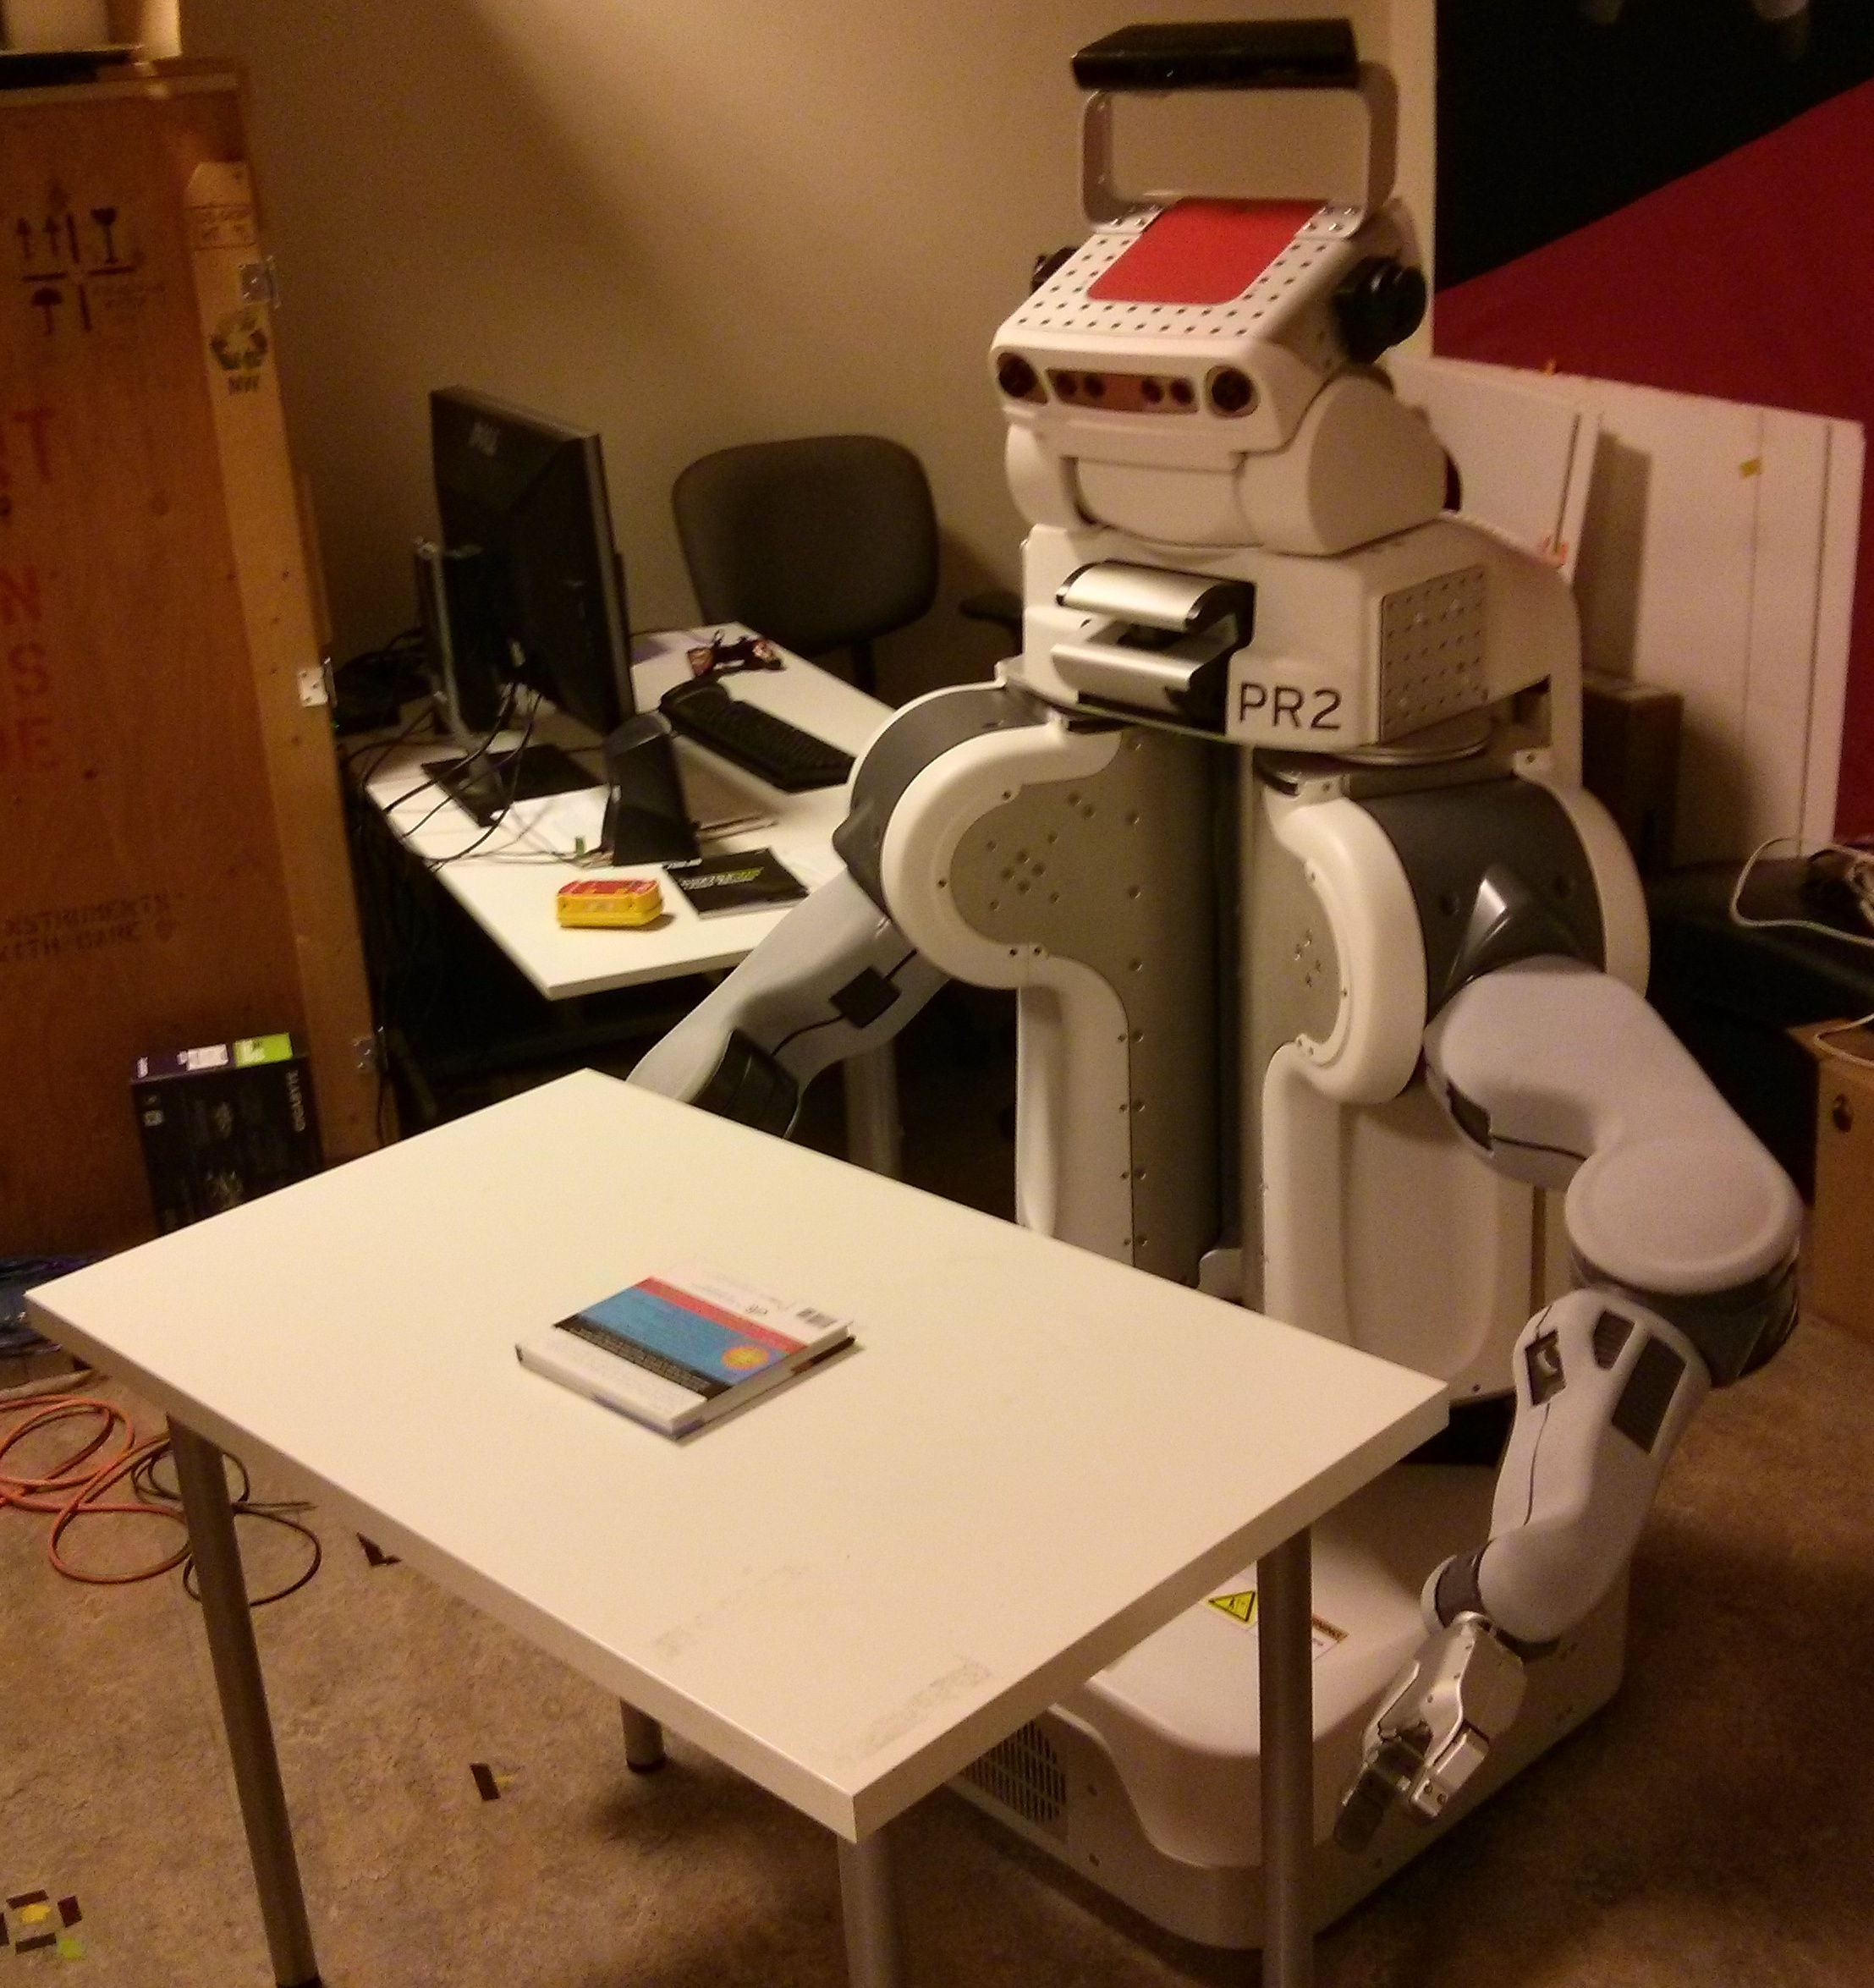
\includegraphics[width=0.46\columnwidth]{pics/pr2_init.jpg}}} & 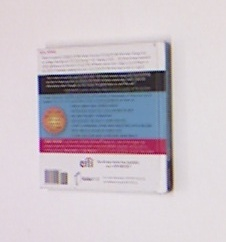
\includegraphics[width=0.23\columnwidth]{pics/first_back.jpg} 
&
\includegraphics[width=0.23\columnwidth]{pics/first_cover1.jpg} \\
\multicolumn{2}{c}{} & 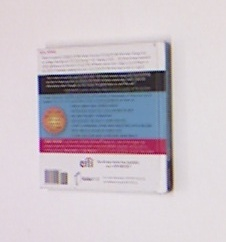
\includegraphics[width=0.23\columnwidth]{pics/first_back.jpg} 
&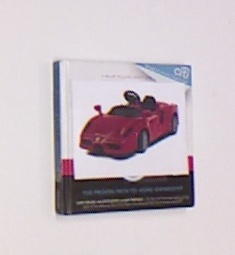
\includegraphics[width=0.23\columnwidth]{pics/first_cover2.jpg} \\
\multicolumn{2}{c}{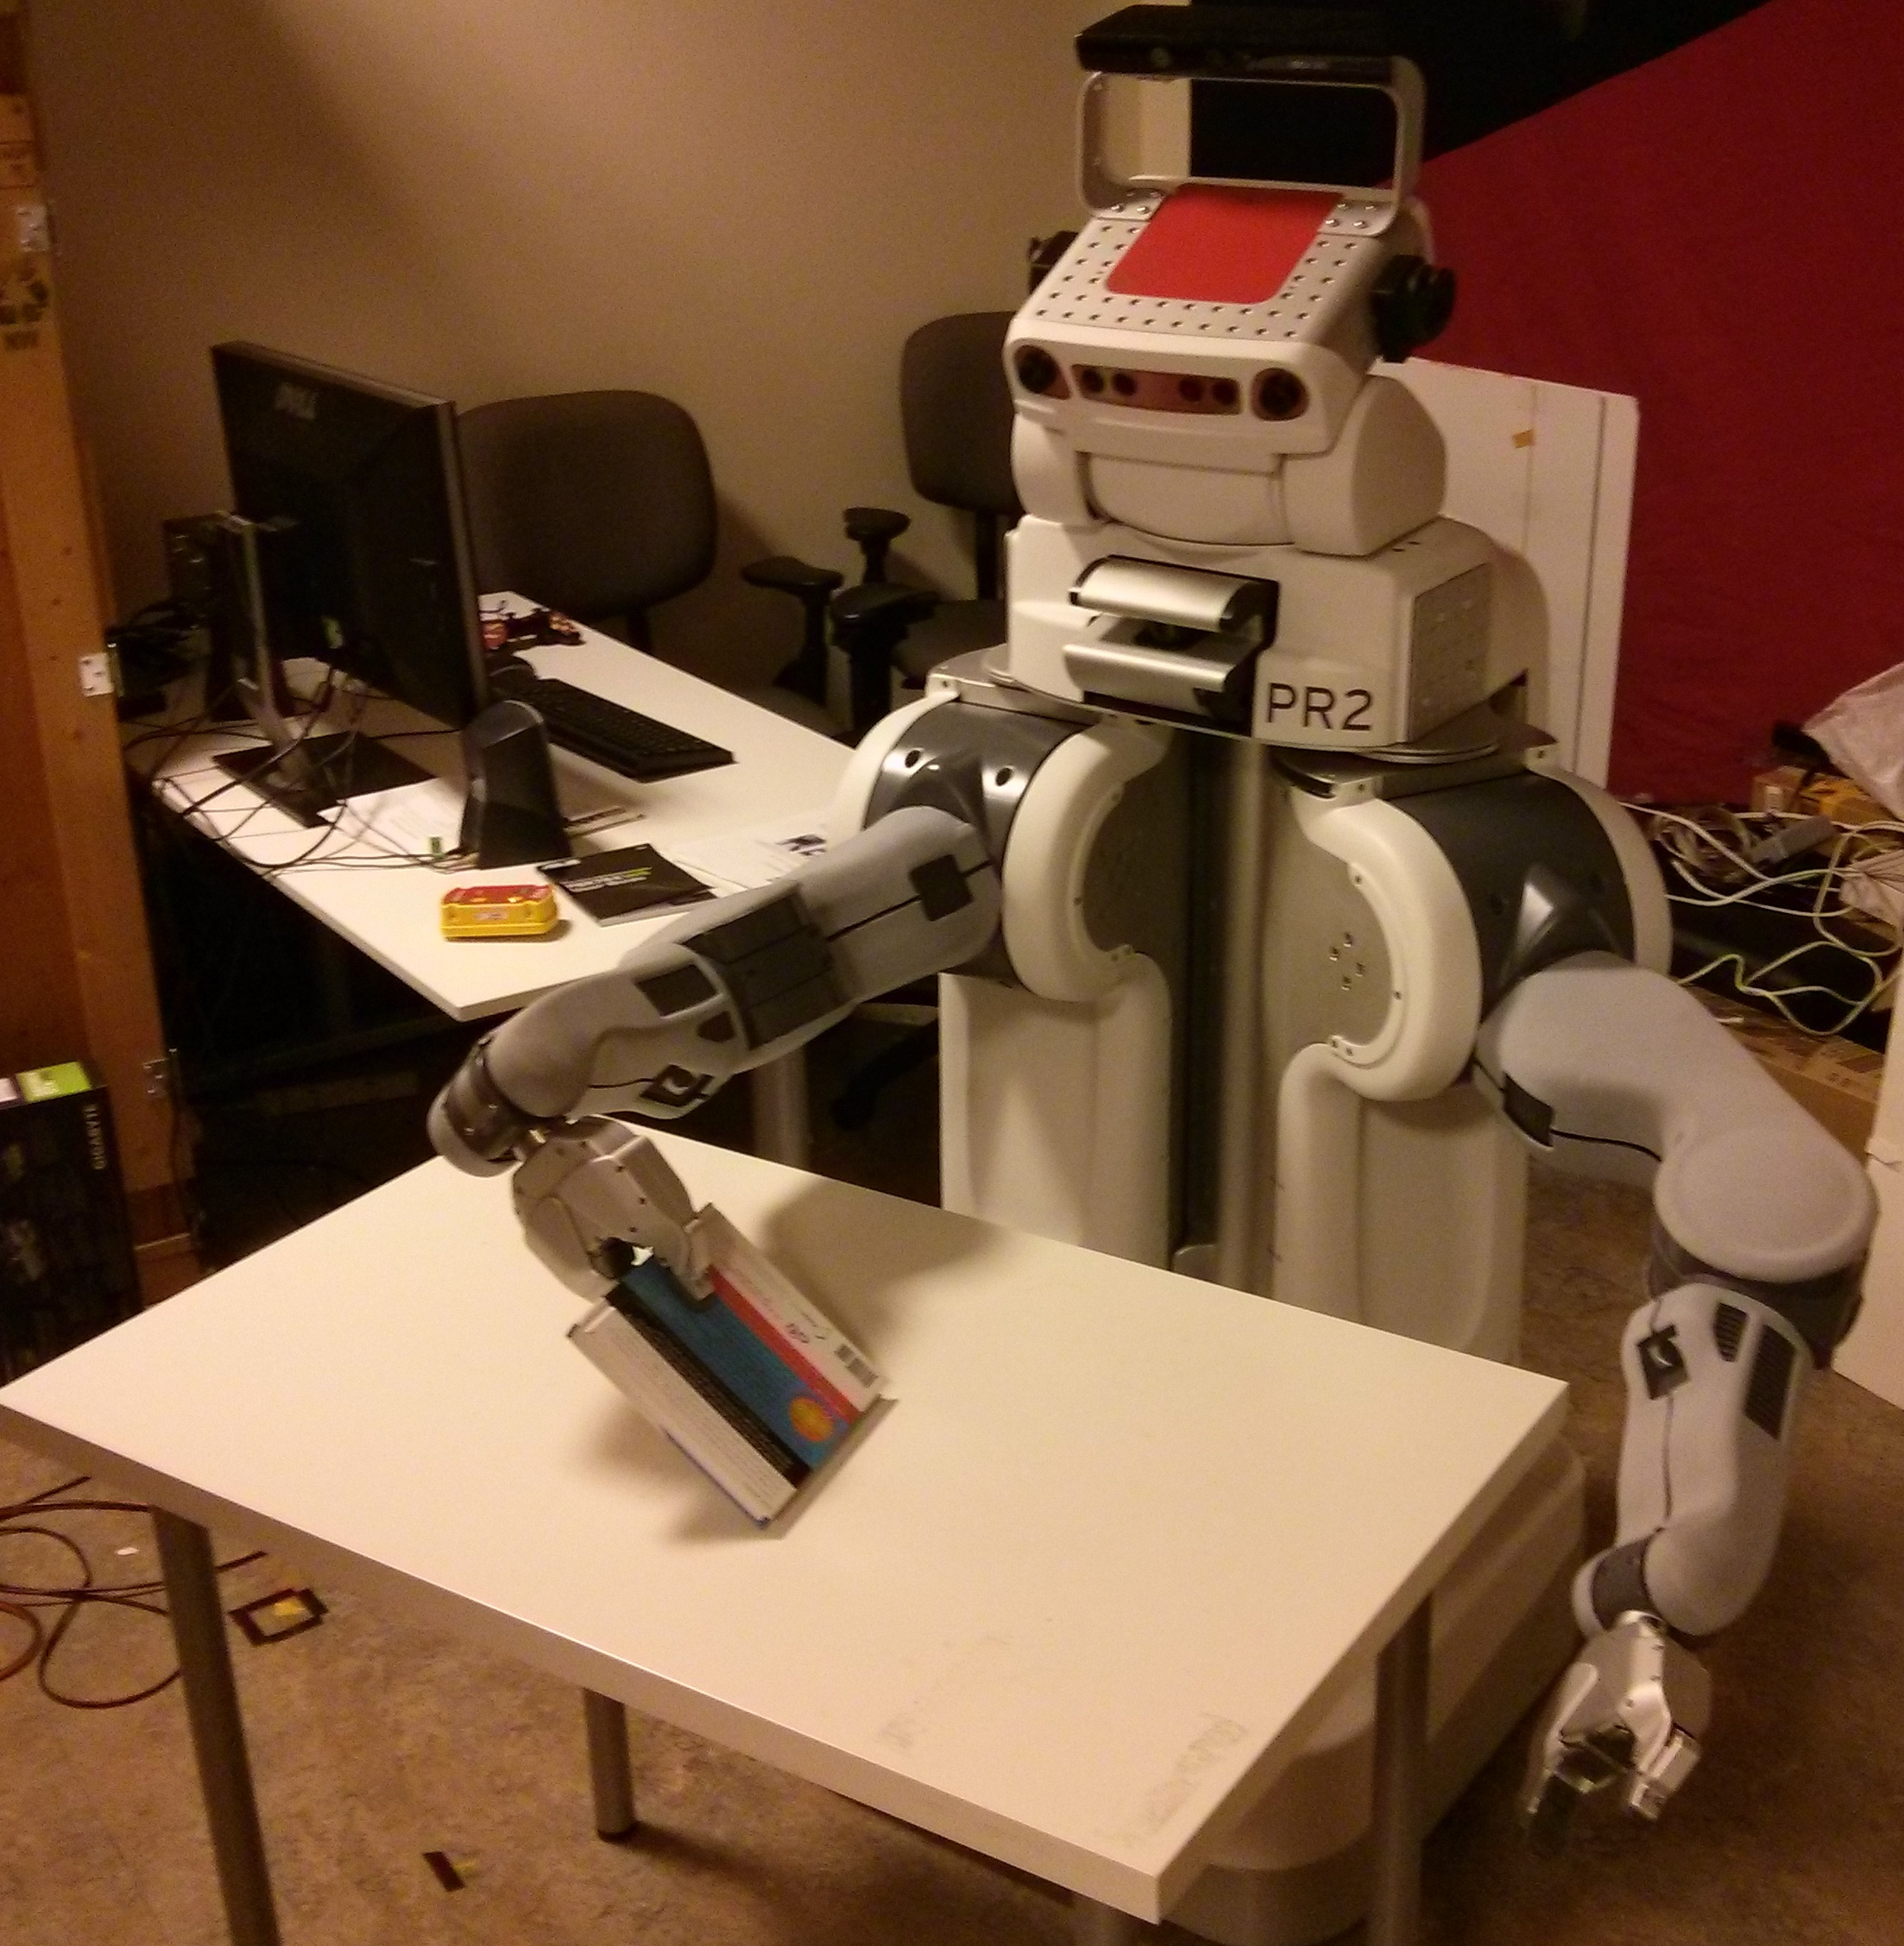
\includegraphics[width=0.45\columnwidth]{pics/pr2_grasp.jpg}}
& \multicolumn{2}{c}{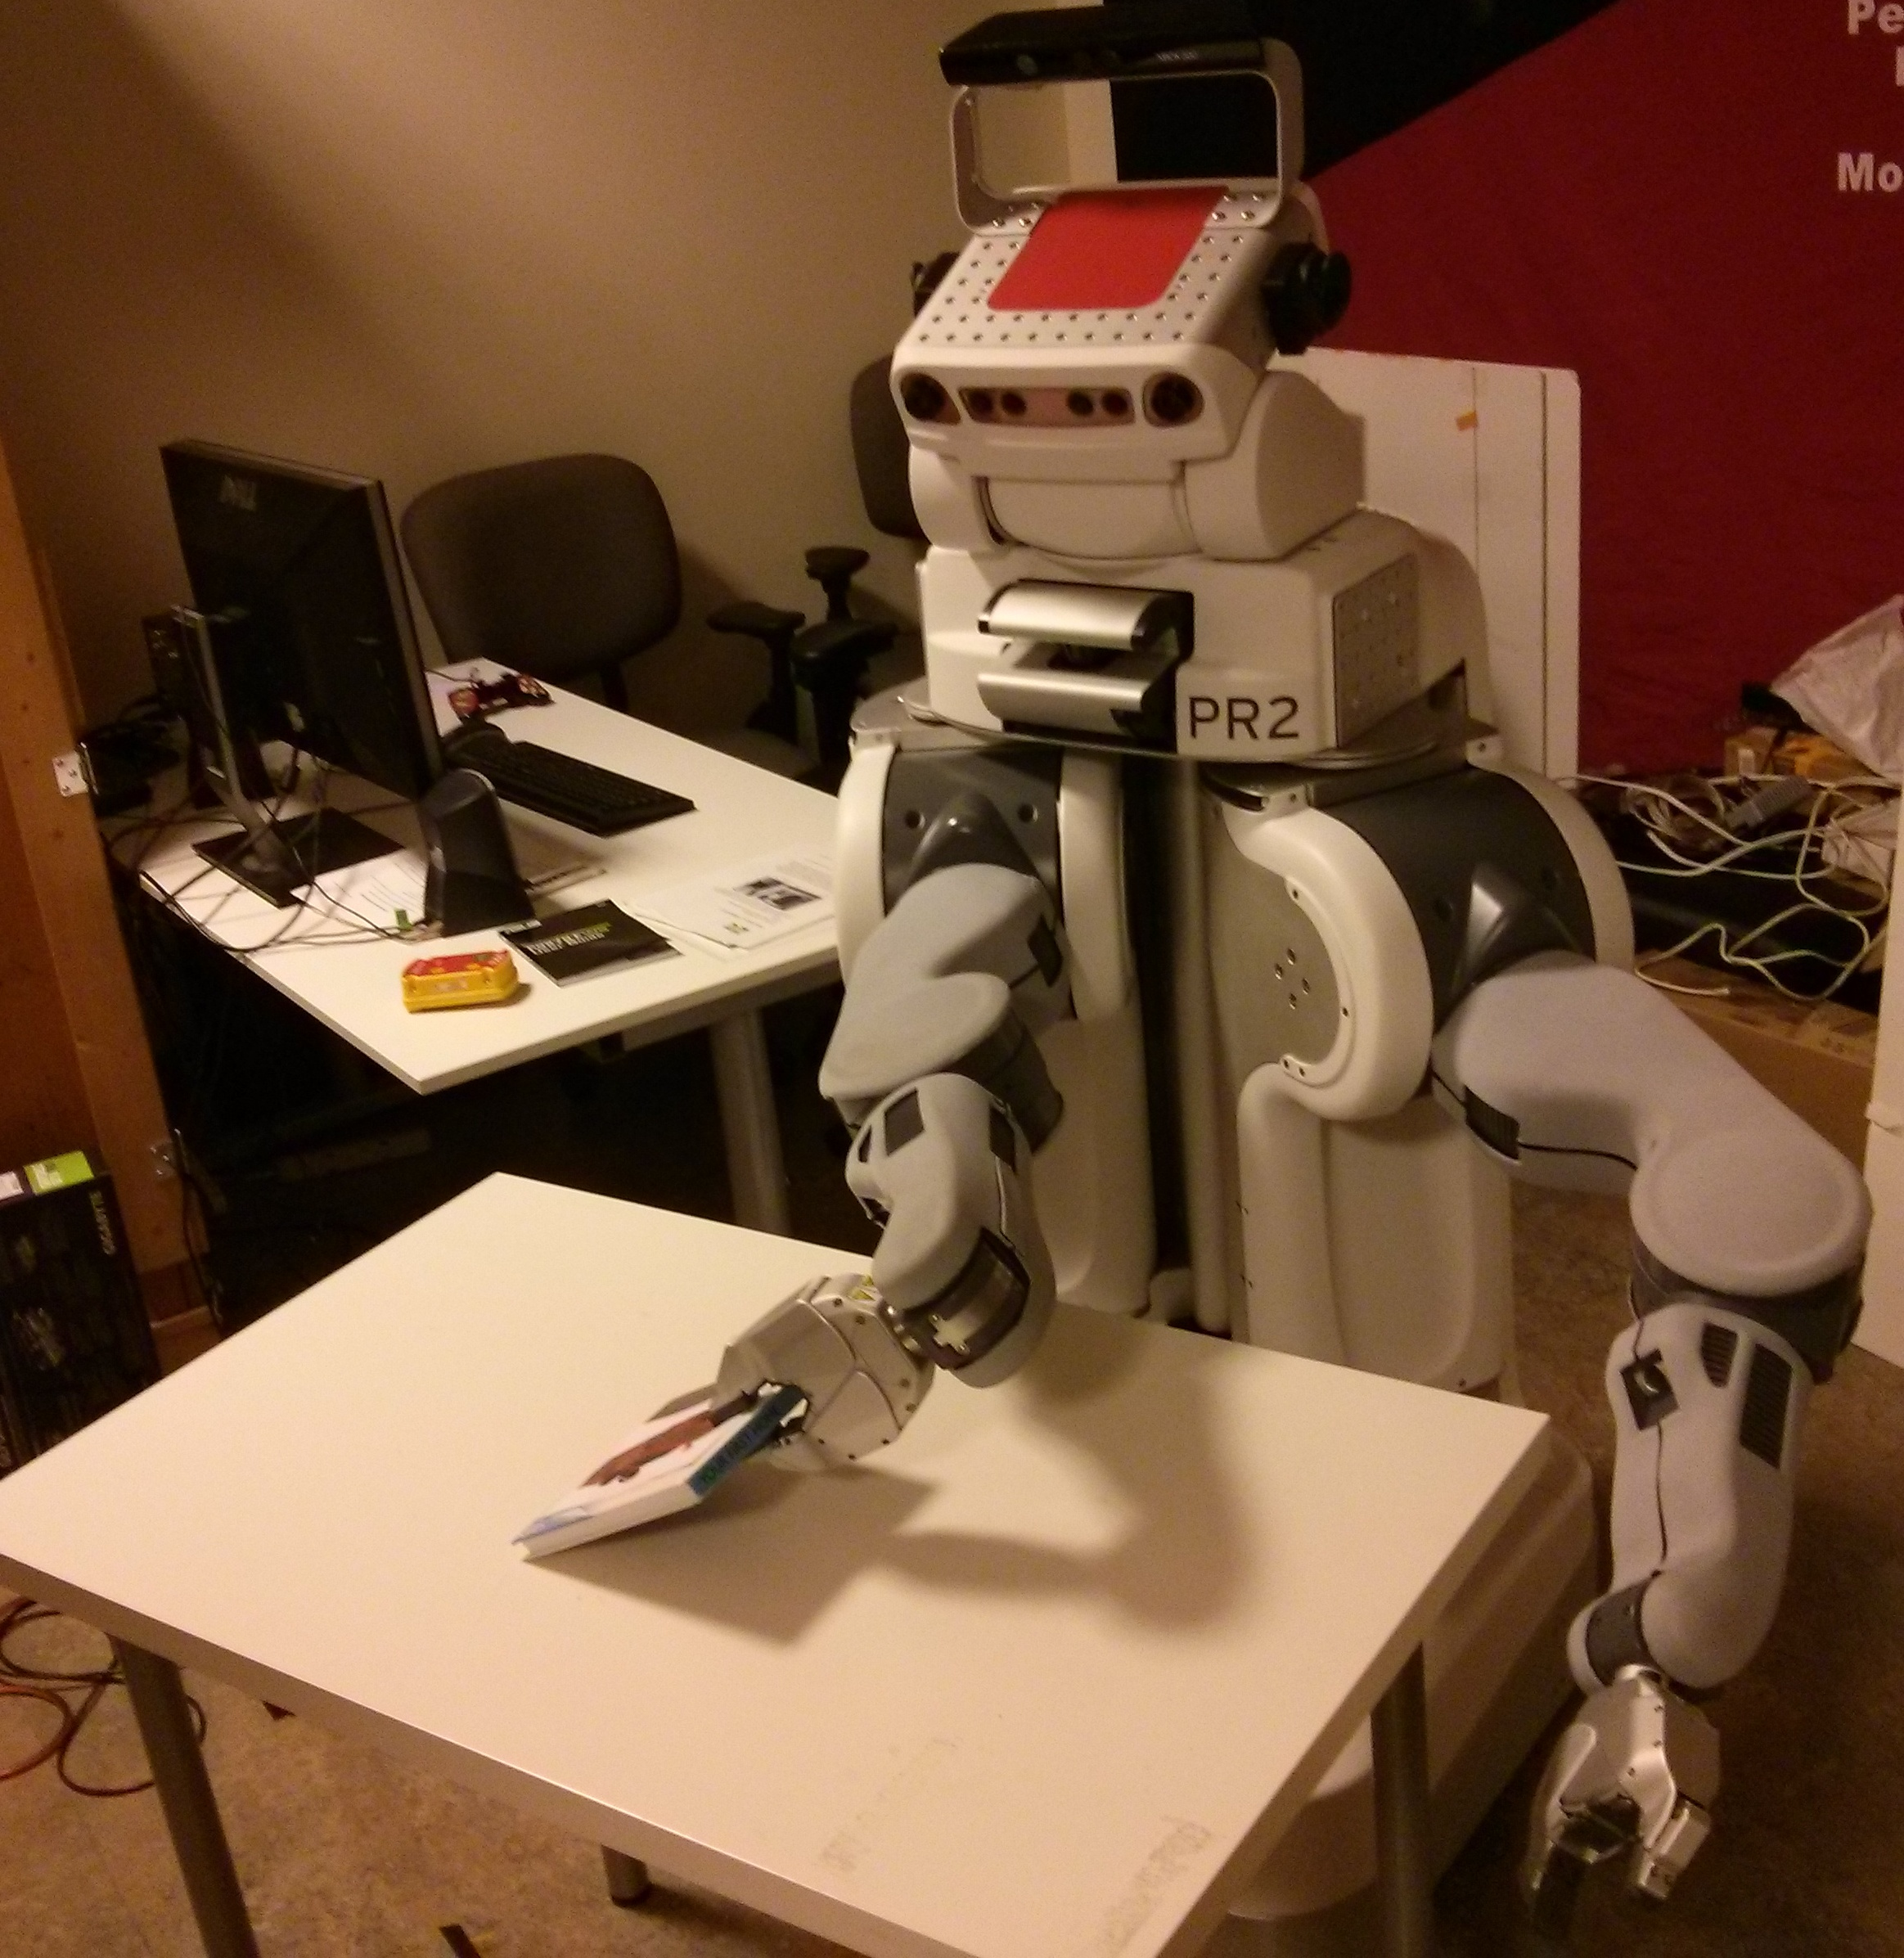
\includegraphics[width=0.45\columnwidth]{pics/pr2_rotate.jpg}}
\end{tabular}
\caption{Top-left: The service robot PR2 trying to recognize a book based on the back. Database of objects consists of book 1 (top-right, NE and NW) and book 2, (top-right, SE and SW) that look the same from the back. PR2 has to take the optimal action in order to recognize which book it is. In this case it means it flips it over(bottom-left, bottom-right).}
\label{fig:pr2}
\end{figure}

%contributions
%* novel probabilistic model for object recognition
%* action selection probabilistic algorithm to pick the optimal action in order to recognize the object

\section{Related Work}

%* object recognition
%* interactive perception
%* interactive segmentation
%* maybe something about expected entropy?


% static object recognition intro
	Research in perception has traditionally focused on  static 
images and recognized objects based on a set of visual features  such as SIFT~\cite{lowe2004distinctive}, SURF~\cite{bay2006surf} or ORB~\cite{rublee2011orb}.
There has also been plethora of work on static object recognition that resulted in various systems.
	
% examples of static object recognition systems	
	One of the most efficient and robust object recognition systems was developed by Tang et al.~\cite{tang2012textured}. The authors use color model matching and SIFT feature matching to recognize the object. The algorithm also performs geometric pose estimation as well as final scene verification and refinement using global scene consistency checks. 

A different approach was discussed by Weijer and Khan~\cite{van2013fusing} where the authors compare various bag-of-words based recognition algorithms. The algorithm represents an image as a set of local regions where each of them is represented as a visual vocabulary. Different objects correspond to different histograms (called bags-of-words) over the created vocabulary. An extracted bag-of-words histogram can be compared to all the histograms stored in the memory and thus, an object can be labelled as one of the previously seen objects.

Although being very successful both of these approaches would not be able to recognize the correct object presented in~\figref{fig:pr2}. That is why we incorporate robot's manipulation capabilities to solve that problem.

%intro to interactive segmentation
The idea of a robot interacting with the scene to improve its perceptual skills has been particularly explored in the area of interactive segmentation.

%interactive segmentation
Segmentation of rigid objects from a video stream 
of objects being moved by a robot has been first addressed by Fitzpatrick et. al.~\cite{fitzpatrick_active_vision} and Kenney et. al.~\cite{KenneyInteractive}.
Katz and Brock~\cite{Katz-WS-MM-ICRA2011} address
the problem of segmenting the articulated objects. Another technique was presented by \cite{bergstrom11icvs}, where the authors propose  an   approach  to
interactive  segmentation that  requires initial  labeling using  a 3D
segmentation  through  fixation  which  results  in  a  rough  initial
segmentation. The robot interacts with the scene to disambiguate
the hypotheses.

%something about methods using expected entropy?

%our work intro interactive object recognition
All these approaches do not take into consideration action choices, action is assumed to be known and performed either by a human or a robot. In this work we introduce a probabilistic method to choose the best action based on robot's observations. To the best of our knowledge, the problem of interactive object recognition has not been addressed before. 


\section{Approach}
give an overview what we will show

\subsection{Object Recognition Model}
\begin{itemize}
\item present the small graph for features, objects and poses
\item present the equations for the graph
\item explain our features
\item plot showing the matching idea
\item plot of training features
\end{itemize}

\subsection{Action Selection Model}
\begin{itemize}
\item present the full graph
\item present the expected entropy equation
\item present the derivations for our reasoning
\end{itemize}

\section{Experimental Results}
\begin{itemize}
\item explain our dataset
\item show pictures of objects
\item show cross validation results for our training
\item explain the setup
\item show real data results for object recognition (table)
\item discuss the results, emphasize that the action selection works
\end{itemize}

\section{Conclusions}
\begin{itemize}
\item discuss the results
\item what failed what succeeded
\item talk about possible extensions: continuous pose, more feature types, on the robot
\end{itemize}

\section*{Acknowledgments}

\cite{McGeer01041990}




%% Use plainnat to work nicely with natbib. 

\bibliographystyle{plainnat}
\bibliography{references}

\end{document}


